\documentclass[12pt]{article}
\usepackage{graphicx}
\usepackage{color}

\begin{document}
\begin{titlepage}
\begin{center}
\begin{huge}
\begin{center}
\textcolor{blue}{V3D Digraph Visualizer Documentation}
\end{center}
\end{huge}
\hfill \break
\begin{Large}
\begin{center}
\textcolor{blue}{Team: App-Synth}
\end{center}
\end{Large}
\begin{small}
\begin{flushleft}
Author(s):
\end{flushleft}

\begin{itemize}
	\item Kulani Bamuza \\
	\item Keanan Jones \\
	\item Munyaradzi Mpofu\\
	\item Neo Thokoa\\	
	\item Takalani Sigama\\
	
\end{itemize}
\end{small}

\end{center}
\begin{center}
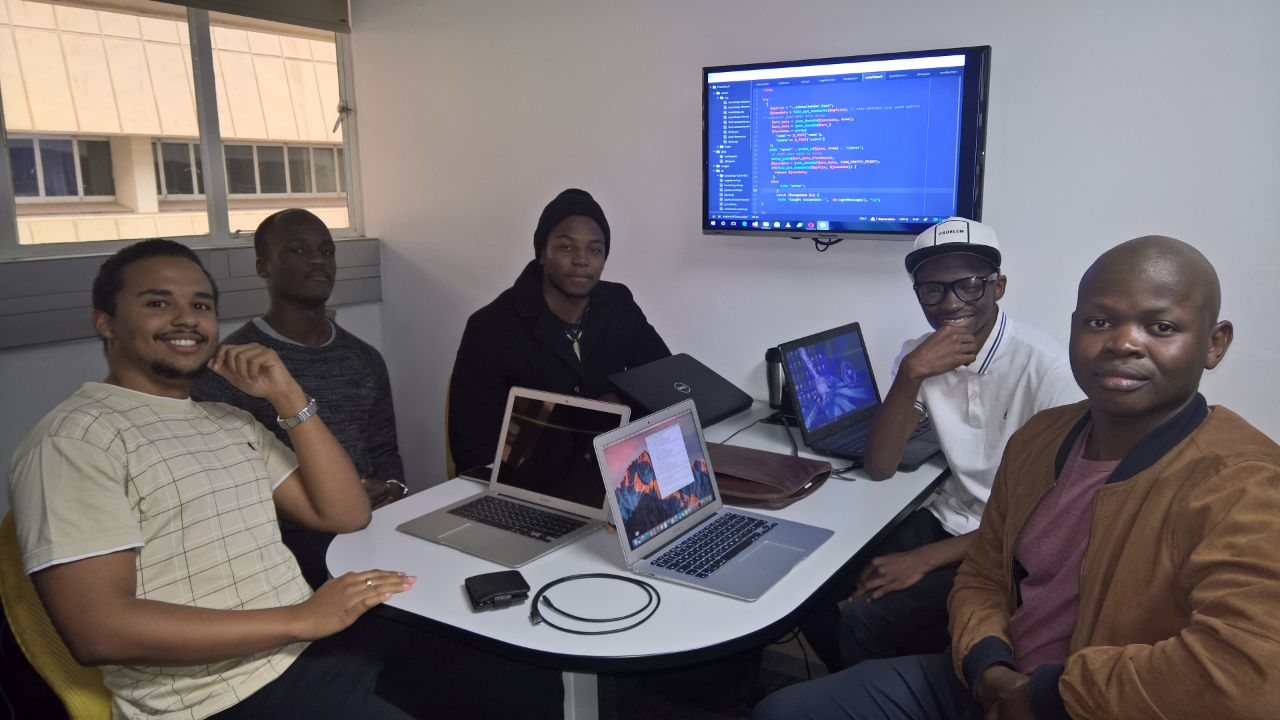
\includegraphics[scale=0.4]{Dps/TeamPic.jpg}
\\
\textcolor{blue}{\textit{University of Pretoria, Department of Computer Science
\\
15 May 2017}}

\end{center}
\end{titlepage}

\newpage
\pagenumbering{arabic}
\thispagestyle{empty}
\tableofcontents
\clearpage

\textcolor{blue}{\section{Agile Documentation}}
\begin{flushleft}
	This document is based on the lecture held by industry expert Justine de Bryne at The University of Pretoria. We aim to follow the quality example displayed by her.
\end{flushleft}

\textcolor{blue}{\section{User Stories}}
\begin{flushleft}
	The user requirements are derived from a number of user stories. This section serves as a reference to the constructed user stories and under which module they fall under.	
	
	\textcolor{blue}{\subsection{Data Module}}	
	\begin{flushleft}
	\begin{itemize}
	\item As a User, I want to Save Graph for later use
	\item As a User, I want to Update Graph during interaction
	\item As a User, I want to Create Graph from a text file to create a model
	\end{itemize}	
	\end{flushleft}
	
	\textcolor{blue}{\subsection{Interaction Module}}	
	\begin{flushleft}
	\begin{itemize}
	\item As a User, I want to Select Vertex in order to move/edit
	\item As a User, I want to Create Vertex to add to the model
	\item As a User, I want to Update Vertex to a new value
	\item As a User, I want to Remove Vertex from the model
	\item As a User, I want to Create Edge add to the model
	\item As a User, I want to Update Edge to modify forces between vertices to observe structural changes
	\item As a User, I want to Remove Edge from the model
	\end{itemize}	
	\end{flushleft}
	
	\textcolor{blue}{\subsection{Rendering Module}}	
	\begin{flushleft}
	\begin{itemize}
	\item As a User, I want to Render VR Graph for viewing
	\item As a User, I want to Reload Graph to diaplay updated version
	\item As a User, I want to Undo Changes made to graph
	\item As a User, I want to Render Graph on External Display for 3rd party user to view
	\end{itemize}	
	\end{flushleft}
	
	\textcolor{blue}{\subsection{Synchronization Module}}	
	\begin{flushleft}
	\begin{itemize}
	\item As a User, I want to Publish State Changes to sync with external display
	\item As a User, I want to Receive State Changes to sync with VR display
	\end{itemize}	
	\end{flushleft}
	
	
\end{flushleft}

\textcolor{blue}{\section{Product Requirements}}
\begin{flushleft}

	Taking the the user stories in to consideration we will now create a set of product requirements. Each requirement we aim to meet within a sprint (a specified number of days).
	
	\textcolor{blue}{\subsection{Data Module}}	
	\begin{flushleft}
	\begin{itemize}
	\item Read graph data in all specified formats
	\item Format the data in such a way that it is easily interpreted for graph construction
	\item Take graph information and export it to a specified file format
	\end{itemize}	
	\end{flushleft}
	
	\textcolor{blue}{\subsection{Interaction Module}}	
	\begin{flushleft}
	\begin{itemize}
	\item Update graph information through graph interaction
	\item Provide undo functionality on graph
	\end{itemize}	
	\end{flushleft}
	
	\textcolor{blue}{\subsection{Rendering Module}}	
	\begin{flushleft}
	\begin{itemize}
	\item Take formatted graph information and construct a graph
	\item Provide real time rendering from user interactions
	\end{itemize}	
	\end{flushleft}
	
	\textcolor{blue}{\subsection{Synchronization Module}}	
	\begin{flushleft}
	\begin{itemize}
	\item Provide real time rendering on viewer based on VR view
	\item Push relevant changes to external viewers
	\end{itemize}	
	\end{flushleft}

\end{flushleft}

\textcolor{blue}{\section{Business Value vs Technical Difficulty \& Product Backlog}}
\begin{flushleft}
 	
 	The product requirements are plotted on the following graph to illustrate how important they are for business success and how difficult each is to implement.
	
	\includegraphics[scale=0.5]{"Deployment Diagrams/businessValueVsTechnicalDifficulty".png}
	
	According to the diagram and fulfilling as many prerequisites as possibly while maintaining concurrency we have the following implementation order on the product backlog.
	
	\includegraphics[scale=0.6]{"Deployment Diagrams/productBacklog".png}

\end{flushleft}

\end{document}